\documentclass{beamer}


\mode<presentation>
{
  \usetheme{Darmstadt}
  \useoutertheme{infolines}
}

\usepackage{alltt}

\usepackage{etex}         % to avoid compilation erros of xypic
\usepackage[curve]{xypic}
%\xyoption{pdf}
%\usepackage[pdf]{xy}


\usepackage[utf8]{inputenc}
\usepackage{proof}
\inferLineSkip=4pt  % increase spacing between lines; default is 2pt

\usepackage{amsmath}
\usepackage{amssymb}
\usepackage{fontawesome}
\usepackage{times}
\usepackage[T1]{fontenc}
\usepackage{listings}
\lstset{language=haskell,basicstyle=\ttfamily}

\usepackage{multicol}
\usepackage{mathpartir}
\usepackage{mathtools}
\usepackage{stmaryrd}
\usepackage{soul}
\usepackage{tikzsymbols}

% Delete this, if you do not want the table of contents to pop up at
% the beginning of each subsection:
\AtBeginSection[]
{
  \begin{frame}<beamer>
    \frametitle{Plan}
    \tableofcontents[sectionstyle=show/shaded,subsectionstyle=hide]
  \end{frame}
}

\AtBeginSubsection[]
{
  \begin{frame}<beamer>
    \frametitle{Plan}
    \tableofcontents[sectionstyle=show/hide,subsectionstyle=show/shaded/hide]
%    \tableofcontents[subsectionstyle=show/shaded/hide]
  \end{frame}
}

\setbeamertemplate{footline}
{%
%\begin{beamercolorbox}{section in head/foot}
%\vskip2pt\insertnavigation{\paperwidth}\vskip2pt
%\end{beamercolorbox}%
\insertpagenumber
\insertshorttitle[width={5cm},center]
\insertshortinstitute[width={3cm},center]
\insertshortdate[width={3cm},center]
}


% If you wish to uncover everything in a step-wise fashion, uncomment
% the following command: 

%\beamerdefaultoverlayspecification{<+->}

\usepackage{tikz}
\usetikzlibrary{trees}
\usetikzlibrary{arrows}
\usetikzlibrary{decorations.pathmorphing}
\usetikzlibrary{shapes.multipart}
\usetikzlibrary{shapes.geometric}
\usetikzlibrary{calc}
\usetikzlibrary{positioning} 
\usetikzlibrary{fit}
\usetikzlibrary{backgrounds}
\usetikzlibrary{automata}


%%% Local Variables: 
%%% mode: latex
%%% TeX-master: "main"
%%% End: 

% Theorems and definitions

% \newtheorem{definition}{Definition}
% \newtheorem{theorem}{Theorem}
% \newtheorem{lemma}{Lemma}
% \newtheorem{proposition}{Proposition}


% Definition of colors
\newcommand{\blue}[1]{{\color{blue}#1}}
\newcommand{\green}[1]{{\color{green}#1}}
\newcommand{\red}[1]{{\color{red}#1}}
\newcommand{\gray}[1]{{\color{gray}#1}}

% From MSCS file
\newcommand{\eg}{\textit{e.g.\ }}
\newcommand{\etal}{\textit{et al.\ }}
\newcommand{\etc}{\textit{etc}}
\newcommand{\ie}{\textit{i.e.\ }}
\newcommand{\viz}{\textit{viz.\ }}
\newcommand{\wrt}{\textit{w.r.t.\ }}
\newcommand{\lex}{\langle}
\newcommand{\rex}{\rangle}

% Own abbreviations
\newcommand{\secref}[1]{Section~\ref{#1}}
\newcommand{\secrefs}[1]{Sections~\ref{#1}}
\newcommand{\figref}[1]{Figure~\ref{#1}}
\newcommand{\figrefs}[1]{Figures~\ref{#1}}
\newcommand{\pgref}[1]{page~\pageref{#1}}
\newcommand{\theoremref}[1]{Theorem~\ref{#1}}
\newcommand{\theoremrefs}[1]{Theorems~\ref{#1}}
\newcommand{\lemmaref}[1]{Lemma~\ref{#1}}
\newcommand{\exampleref}[1]{Example~\ref{#1}}
\newcommand{\defref}[1]{Definition~\ref{#1}}

\newcommand{\figline}{\rule{\textwidth}{0.5pt}}


% Logique

\newcommand{\IMPL}[0]{\longrightarrow}
\newcommand{\IMPLL}[0]{\Longrightarrow} % another implication, to make
                                % a difference with reduction relations
\newcommand{\AND}[0]{\land}
\newcommand{\OR}[0]{\lor}
\newcommand{\NOT}[0]{\lnot}
\newcommand{\FALSE}[0]{\perp}
\newcommand{\TRUE}[0]{\top}
\newcommand{\IFF}[0]{\leftrightarrow}
\newcommand{\BIGAND}[1]{\bigwedge_{#1}}
\newcommand{\BIGOR}[1]{\bigvee_{#1}}
\newcommand{\BIGANDC}[2]{\bigwedge_{#1|#2}} % bigand with constraint
\newcommand{\BIGORC}[2]{\bigvee_{#1|#2}}    % bigor with constraint

\newcommand{\exgeq}[1]{\exists^{{\geq #1}}}
\newcommand{\exeq}[1]{\exists^{{= #1}}}
\newcommand{\exle}[1]{\exists^{{< #1}}}

% Other

\newcommand{\smalltalcq}[0]{{\small small}-t{$\cal ALCQ$}}
\newcommand{\smalltalcqe}[0]{{\small small}-t{$\cal ALCQ$e}}
\newcommand{\trule}[0]{\xhookrightarrow}
\newcommand{\tableaurule}[1]{{\xhookrightarrow[]{#1}}}
\newcommand{\nodes}[1]{{\cal N}({#1})}
\newcommand{\trans}[1]{{\cal T}({#1})}
\newcommand{\transm}[1]{{\cal T'}({#1})}
\newcommand{\rconts}[1]{\llparenthesis #1 \rrparenthesis} %record contents
\newcommand{\rupd}[2]{{#1}\llparenthesis #2 \rrparenthesis} %record update

\newcommand{\eform}[0]{\mathit{eform}}
\newcommand{\form}[0]{\mathit{form}}
\newcommand{\free}[0]{\mathit{free}}
\newcommand{\exclprop}[0]{\stackrel{\times}{\longrightarrow}}


%----------------------------------------------------------------------
% For drawing syntax diagrams
% ----------------------------------------------------------------------

% Environment defining the general layout

\newenvironment{syntaxdiagram}[1]
{
%  \begin{equation}\label{eq:#1}
  \begin{tikzpicture}[%
node distance=5mm and 10mm,
>=stealth',
black!50,
text=black,
graphs/every graph/.style={edges=rounded corners},
hv path/.style={to path={-| (\tikztotarget)}},
vh path/.style={to path={|- (\tikztotarget)}},
nonterminal/.style={%
rectangle,
minimum size=6mm,
draw=black,
},
terminal/.style={%
rectangle,minimum size=6mm,rounded corners=3mm,
draw=black!50,
},
start/.style={%
circle,inner sep=1pt,minimum size=1pt,fill=white,draw=black!50,
},
end/.style={%
start,
},
junction/.style={circle,inner sep=0pt,minimum size=0pt},]
\node[nonterminal] (#1) {\hypertarget{syn:#1}{#1:}};
}
{\end{tikzpicture}
%\end{equation}
}

% Connects start point #1 via intermediate node entry #2 and exit #3
% to an end point #4.
\newcommand{\syndiagAlternative}[4]{%
\graph[use existing nodes] {
#1 ->[vh path] #2;
#3 ->[hv path] #4;
};
}

% Connects start point #1 via intermediate node #2 (typically a junction)
% to an end point #3.
\newcommand{\syndiagBridge}[3]{%
\graph[use existing nodes] {
#1 --[vh path] #2;
#2 ->[hv path] #3;
};
}

\newcommand{\nonterminalref}[1]{\hyperlink{syn:#1}{#1}}


%----------------------------------------------------------------------
% Remarks
% ----------------------------------------------------------------------

\newcommand{\remms}[2][]{\todo[color=green!40,#1]{MS: #2}}



%%% Local Variables: 
%%% mode: latex
%%% TeX-master: "main"
%%% End: 


\title{Reasoning with and about Rules and Processes}

\author{Avishkar Mahajan and Martin Strecker}
\date{2022-07-14}


%======================================================================

\begin{document}


%======================================================================

\begin{frame}
  \titlepage
\end{frame}



%======================================================================
\section{Reasoning with and about Rules}


%-------------------------------------------------------------
\begin{frame}[fragile]\frametitle{What's the difference?}

  \blue{Reasoning \emph{with} rules:}
  \begin{itemize}
  \item Given:
    \begin{itemize}
    \item A set of rules  (\emph{e.g.: insurance contract})
    \item A specific scenario (\emph{e.g.: dammage / accident})
    \end{itemize}
  \item Sought:
    \begin{itemize}
    \item A judgement (\emph{who pays / how much?})
    \item Possibly with a justification (\emph{why?})
    \end{itemize}
  \end{itemize}

  \vspace{4mm}
  \blue{Reasoning \emph{about} rules:}
  \begin{itemize}
  \item Given:
    \begin{itemize}
    \item A set of rules  (\emph{e.g.: insurance contract})
    \item A notion of rule consistency
    \end{itemize}
  \item Sought:
    \begin{itemize}
    \item \emph{Either} an inconsistent scenario 
    \item \emph{or} a proof of consistency
    \end{itemize}
  \end{itemize}


\end{frame}

%-------------------------------------------------------------
\begin{frame}[fragile]\frametitle{Example: AXA insurance case study - \emph{Rules}}

  \dots{} about the coverage provided for the vehicle breakdown

  \blue{What is covered}
  \begin{itemize}
  \item If the vehicle breaks down more than one mile from your home, we will
    arrange and pay for a breakdown vehicle to come to the vehicle (for up to
    one hour) to try to get it working again.
    
  \item If the vehicle cannot be made safe to drive at the place you have
    broken down, we will arrange for the vehicle, the driver and passengers to
    be recovered to a repairer or a destination of your choice within 20 miles
    of where you have broken down.
  \end{itemize}
  
  \blue{What is not covered}
  \begin{itemize}
  \item A breakdown at or within one mile from your home.  
  \item Travel outside the UK.  
  \end{itemize}


\end{frame}

%-------------------------------------------------------------
\begin{frame}[fragile]\frametitle{Example: AXA insurance case study}

  \blue{Reasoning \emph{with} rules}
  
Is a cover provided for a mechanical breakdown in Swansea (that is 10 miles
away from home)?

\begin{lstlisting}
fact premiumPaid
fact currentSit mechanicalBrkd
fact situationInLocation mechanicalBrkd swansea
fact distance home swansea 10

assert <scen1_assert2> {SMT: valid} 
coverProvided mechanicalBrkd payBreakdownVehicle
\end{lstlisting}
\emph{Answer: Yes}

\end{frame}

%-------------------------------------------------------------
\begin{frame}[fragile]\frametitle{Example: AXA insurance case study}

  \blue{Reasoning \emph{about} rules}
  
  \begin{itemize}
  \item Is the rule set inconsistent?
  \item More precisely: Is there a situation such that the insurance has to
    pay and can refute payment?
  \end{itemize}
  
  \begin{lstlisting}
    for mySit: Situation, myCov: CoverageType
    assert <contradictoryCover> {SMT: consistent}
    coverProvided mySit myCov && myCov /= noCoverProvided &&
    coverProvided mySit noCoverProvided
  \end{lstlisting}
\vspace{-5mm}
  \emph{Answer:} Scenario:
  \begin{lstlisting}
    currentSit mechanicalBrkd
    coverProvided mechanicalBrkd noCoverProvided
    coverProvided mechanicalBrkd payBreakdownVehicle
    isBreakdownSituation mechanicalBrkd
    isIn home uk
    isIn dundalk abroad
    distance home dundalk d =  (15 <= d) && (d < 19)
  \end{lstlisting}
  
\end{frame}


%-------------------------------------------------------------
\begin{frame}[fragile]\frametitle{Evaluation}

  \blue{What's the interest?}
  \begin{itemize}
  \item Sanitize your rules before running them in production mode
  \item Similar to software verification before deployment
  \end{itemize}

  \vspace{4mm}
  \blue{Where are the difficulties?}
  \begin{itemize}
  \item \emph{Input:} Rules and \emph{lots} of everyday knowledge
    \begin{itemize}
    \item Geography
    \item Components of a car
    \item No breakdown in two different locations at the same time
    \end{itemize}
  \item \emph{Input:} Notion of consistency
  \item \emph{Output:} Comprehensible display of scenarios
  \end{itemize}

\end{frame}



%======================================================================
\section{Reasoning with and about Processes}


%-------------------------------------------------------------
\begin{frame}[fragile]\frametitle{Rules and Automata}

  An antagonistic view? \emph{No!}

\blue{Rules} for modelling time-independent situations

\blue{Automata} for modelling time-dependent processes
\begin{itemize}
\item prevalent in today's Business Process Management tools
\item but what about compliance?
\end{itemize}

\begin{columns}
  \column{.5\textwidth}
  \begin{center}
  BPM languages:

    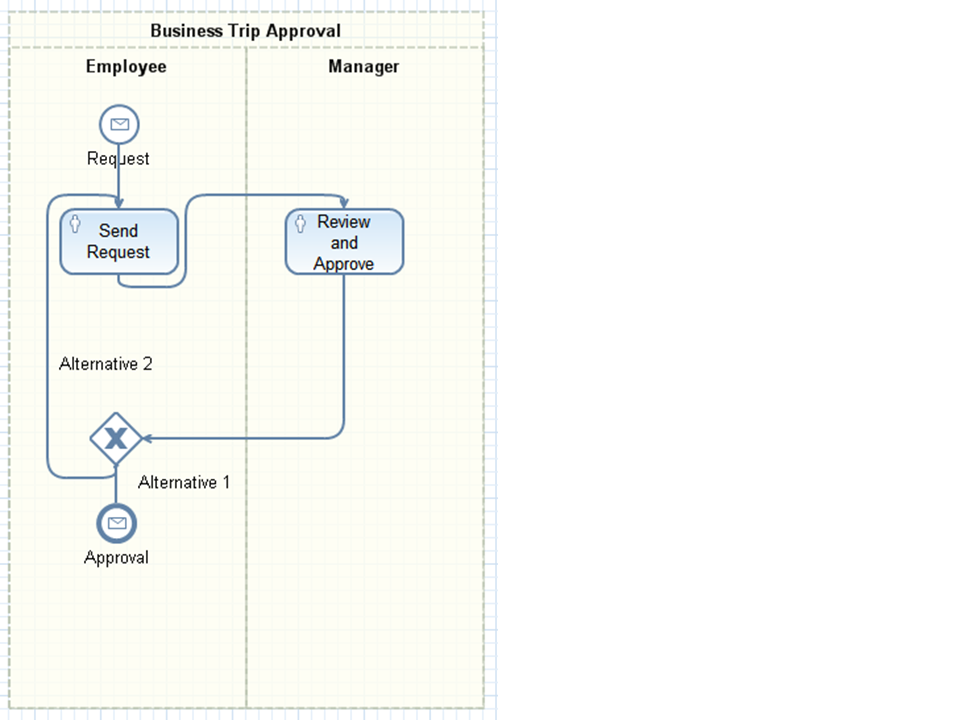
\includegraphics[scale=0.2]{Figures/business_process.png}
    
    \tiny{(from  SAP BPM pages)}
  \end{center}
  \column{.5\textwidth}
  \begin{center}
    Uppaal \red{(live demo!)}
  
    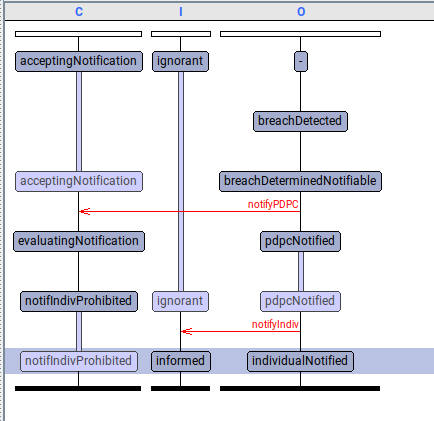
\includegraphics[scale=0.35]{Figures/uppaal_swimlane.png}
  \end{center}
\end{columns}

\end{frame}



%======================================================================
\section{Symbolic AI for the Law}


%-------------------------------------------------------------
\begin{frame}[fragile]\frametitle{Symbolic AI for the Law}

\blue{Main Framework: Logic Programming}
\begin{itemize}
\item Logic programming is a suitable paradigm for symbolic AI and thus can be used for computational law
\item Can naturally incorporate rule priorities/exceptions etc through defeasible reasoning
\end{itemize}

\vspace{4mm}
\blue{Logic Programming based Expert System}
\begin{itemize}
\item Generate questions automatically from a rule set and a query
\item Display justification graph for derived answer
\item Process is fully automated. When rule set changes so do the questions
\end{itemize}

\end{frame}



%-------------------------------------------------------------

\end{document}


%%% Local Variables: 
%%% mode: latex
%%% TeX-master: t
%%% coding: utf-8
%%% End: 
